\chapter{Completion in Pharo}
\label{chap:Completion in Pharo}

In this chapter, we give a detailed overview of the implementation details behind the current completion engine in the Pharo IDE, challenges of code completion for a dynamically typed language, as well as describe the idea behind the sorter plugin.

\section{Code Completion Background}
So, first things first. The Pharo programming language is an object-oriented dynamically typed programming language with a Smalltalk-like syntax. The Pharo IDE is a programming environment meant specifically for developing in Pharo. You have a virtual machine (VM), on top of which an image can be run, which, referencing other IDEs, sort of serves as the current IDE workspace.

The interesting thing here is that the Pharo IDE itself is written in Pharo, and can be extended from within. This means, for example, that when implementing code completion, you can be testing it live in the very environment where you are developing it, which, of course, if not done carefully, can lead you to breaking the image. However, this pecularity is still is an immense advantage with a project like this.

Going deeper into how the completion in the Pharo IDE works, we will explain several important details that are needed to understand the rest of this work. Firstly, code completion is called at every keystroke after we have two and more alphabetic characters in a token. We create a completion context for all the text typed up until then, be it in the Playground or in the Editor. (Essentially, the Playground is a tool for generating small scripts and sketching out some code, whereas the Editor is where you write and edit code for a particular method of a class, i.e. the place to implement the functionality of your classes; see figures \ref{fig:playground} and \ref{fig:editor}).

The completion context parses the text and transforms it into the AST representation, such as a sequence of AST nodes. In the process all the information needed for further actions is extracted: for example, we get the currect position of the cursor (i.e. where we want to get the completion) and the class where we are currently operating (or information that it's in the Playground). Doing the semantic analysis, we get the most fitting type of node for each part of code, and then go to each node to get the correct completion behaviour. For instance, this means that for a Global node, we want to be suggested all the globals, such as class names, for a Message node we only want to get message sends to a variable (in other words, method calls applicable to a certain class instance), and so on.

\begin{figure}[H]
    \centering
    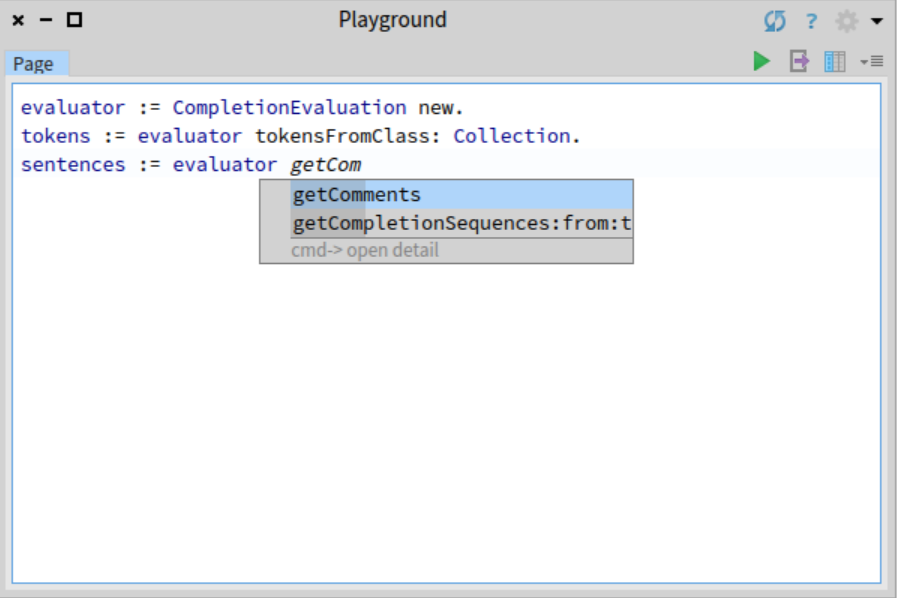
\includegraphics[width=0.9\linewidth]{images/completion1.png}
    \caption{Completion in the Playground}
    \label{fig:playground}
\end{figure}

\begin{figure}[H]
    \centering
    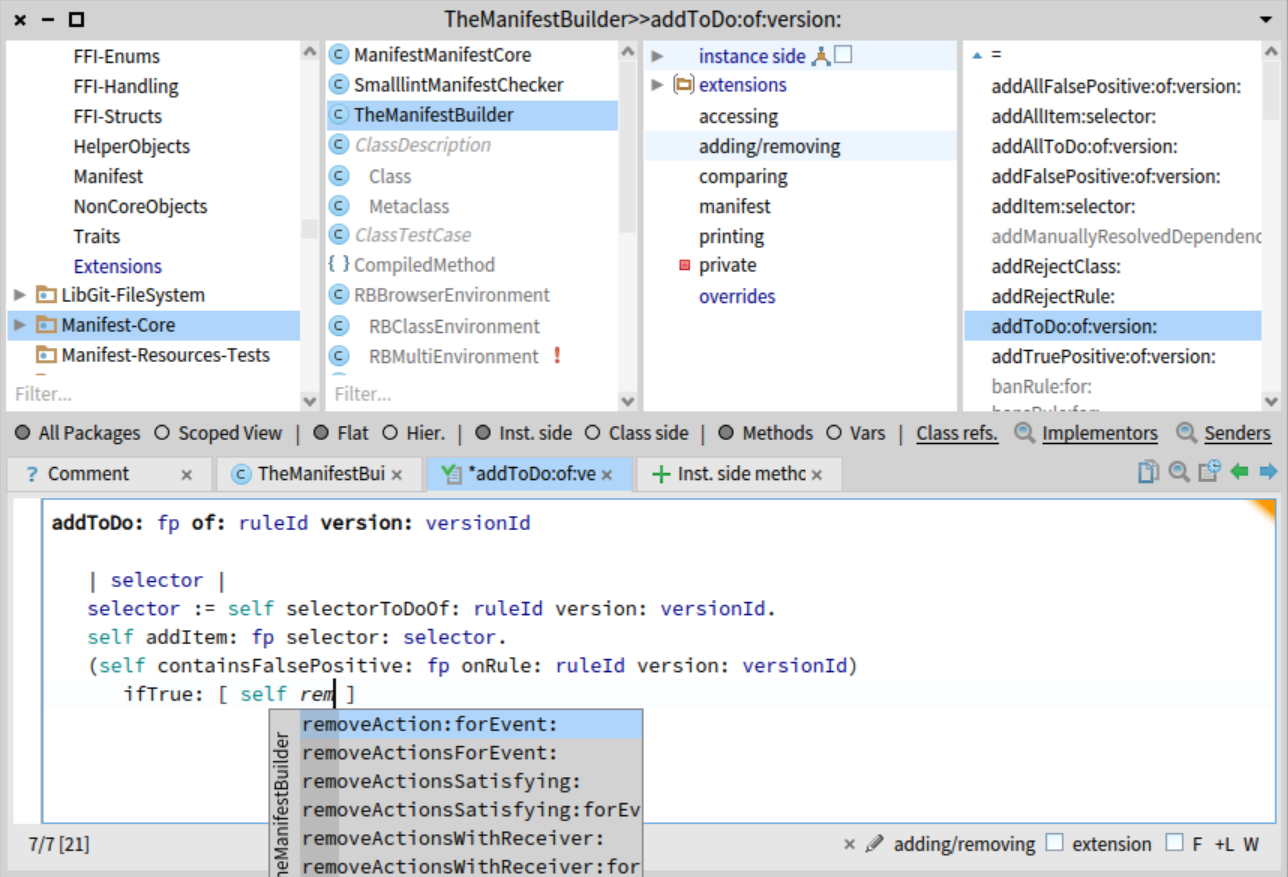
\includegraphics[width=0.9\linewidth]{images/completion2.png}
    \caption{Completion in the Editor}
    \label{fig:editor}
\end{figure}

Therefore, combining the available symbol prefix of length 2 and more that we have, as well as relevant semantic information, we are able to give a list of fitting completion suggestions that are then passed into a sorter and, in the default Pharo IDE completion, are sorted alphabetically. The list itself is displayed in a completion menu that pops up once the completion is called and then is updated with every new keystroke, unless the developer cancels it by pressing \textit{Esc} or clicking to the side of the text area. The completion window can also disappear once we've entered the error node, i.e. the developer mistyped something and there are no valid suggestions to give anymore.

\section{Sorter Plugin}
With Pharo being a dynamically-typed language, however, the semantic analysis of source code is a little tricky. Mainly because more often than not, we are unable to extract type information, as very often it is not yet known at the moment of typing. This makes the completion suggestions that are given for something like message sends appear too general, and often the specific completion the developer has in mind can be too far down the list of suggestions. In the end, this is ineffective, as it requires scrolling through the suggestions list, or typing more characters. But there is one silver lining: even at the beginning knowing that the alphabetic sort would not be accurate enough, we implemented a sorter plugin.

The sorter plugin is technically a part of the completion but it's implemented separately and is intended for usage even without knowing the details of the completion engine. Specifically, within the sorter we treat the completion implementation as a sort of a black box, and the only information we receive is the list of completions we want to sort. This was done to make the sorter extendable and open for modication by any developer, so one could take the general completion functionality and then on top of it put any sorting strategy they would like to have.

Essentially this means that the way we get the completion results themselves is the same, i.e. we semantically analyse the source code and try to give relevant nodes as precisely as possible. However, the sorting strategy really matters when it comes to tokens where we cannot give any precise suggestions by analysis alone, and displaying them in a certain order, that the developer of the sorting strategy hypothesises to be helpful, can really improve the end result (i.e. the list of suggestions displayed in the pop up completion menu).

Now, our idea, as has been mentioned in the introduction, involves sorting the completion candidates based on trained N-gram models that determine the most likely tokens (by seeing what tokens or pairs of tokens were most frequently used in the code history). This means that, at least for bigrams, additional context will be needed to determine the history, or in this case the token which preceedes the one we are trying to complete. For this context, we need the source code of the method we are in, the cursor position, and so on. Hence, for our idea we need more than just a list of completion candidates, but by adding some extension functionality to the completion engine, we will be able to pass both the context information and the list of completions to the sorter, and we will have all the information available right away exactly where we need it.